\section{Evaluation}
\label{sec:eva}

Besides introduction of \textit{Preprocessing} and adaptions in \textit{Bundling}, post hoc bundling evaluation methods are also developed in RAEB.
This section introduces these methods, including mutual information and bundle deviation measurements.

%%%%%%%%%%%%%%%%%%%%%%%%%%%%%%%%%%%%%%%%%%%%%%%%%%%%%%%%%%%%%%%%%%%%%%%%%%%%%%%%%%%%%%%%%%%%%%%%%%
\subsection{Normalized Mutual Information}
After each bundling iteration, a bundling method needs to decide whether the bundling iteration should continue or not.
KDEEB presets a bundling iteration parameter $p_n$, similar to many other bundling methods including SBEB, FTTEB, and CUBu.
$p_n$ = 10 is chosen such that the bundles converge to a stable structure.
Structure stability is basically the perception of visual similarity between images generated in two consecutive bundling iterations.
However, the perception can be easily biased by many factors, including people's color perception difference, lighting conditions, etc.
It lacks a quantitative method for measuring structure stability.

\begin{figure}[t]
	\centering
	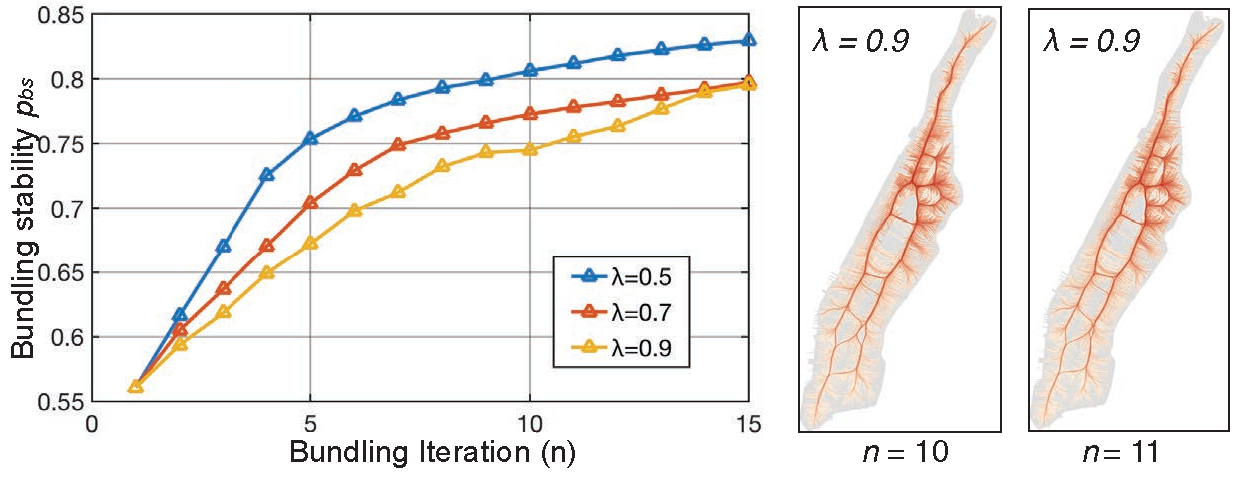
\includegraphics[width=0.495\textwidth]{figure/edgebundling/fig5_NMI/bundle_termination.pdf}
	\vspace{-5mm}
	\caption{(left) Bundling stability $p_{bs}$ measured at each bundling iteration for different decay ratios $\lambda$, (right) visually indistinguishable images are generated at iteration 10 and 11 for $\lambda=0.9$.}
	\label{fig:nmi}
	\vspace{-4mm}
\end{figure}

%%%%%%%%%%%%%%%%%%%%%%%%%%%%%%%%%%%%%%%%%%%%%%%%%%%%%%%%%%%%%%%%%%%%%%%%%%%%%%%%%%%%%%%%%%%%%%%%%%
%%%%%%%%%%%%%%%%%%%%%%%%%%%%%%%%%%%%%%%%%%%%%%%%%%%%%%%%%%%%%%%%%%%%%%%%%%%%%%%%%%%%%%%%%%%%%%%%%%
\begin{figure*}[t]
	\centering
	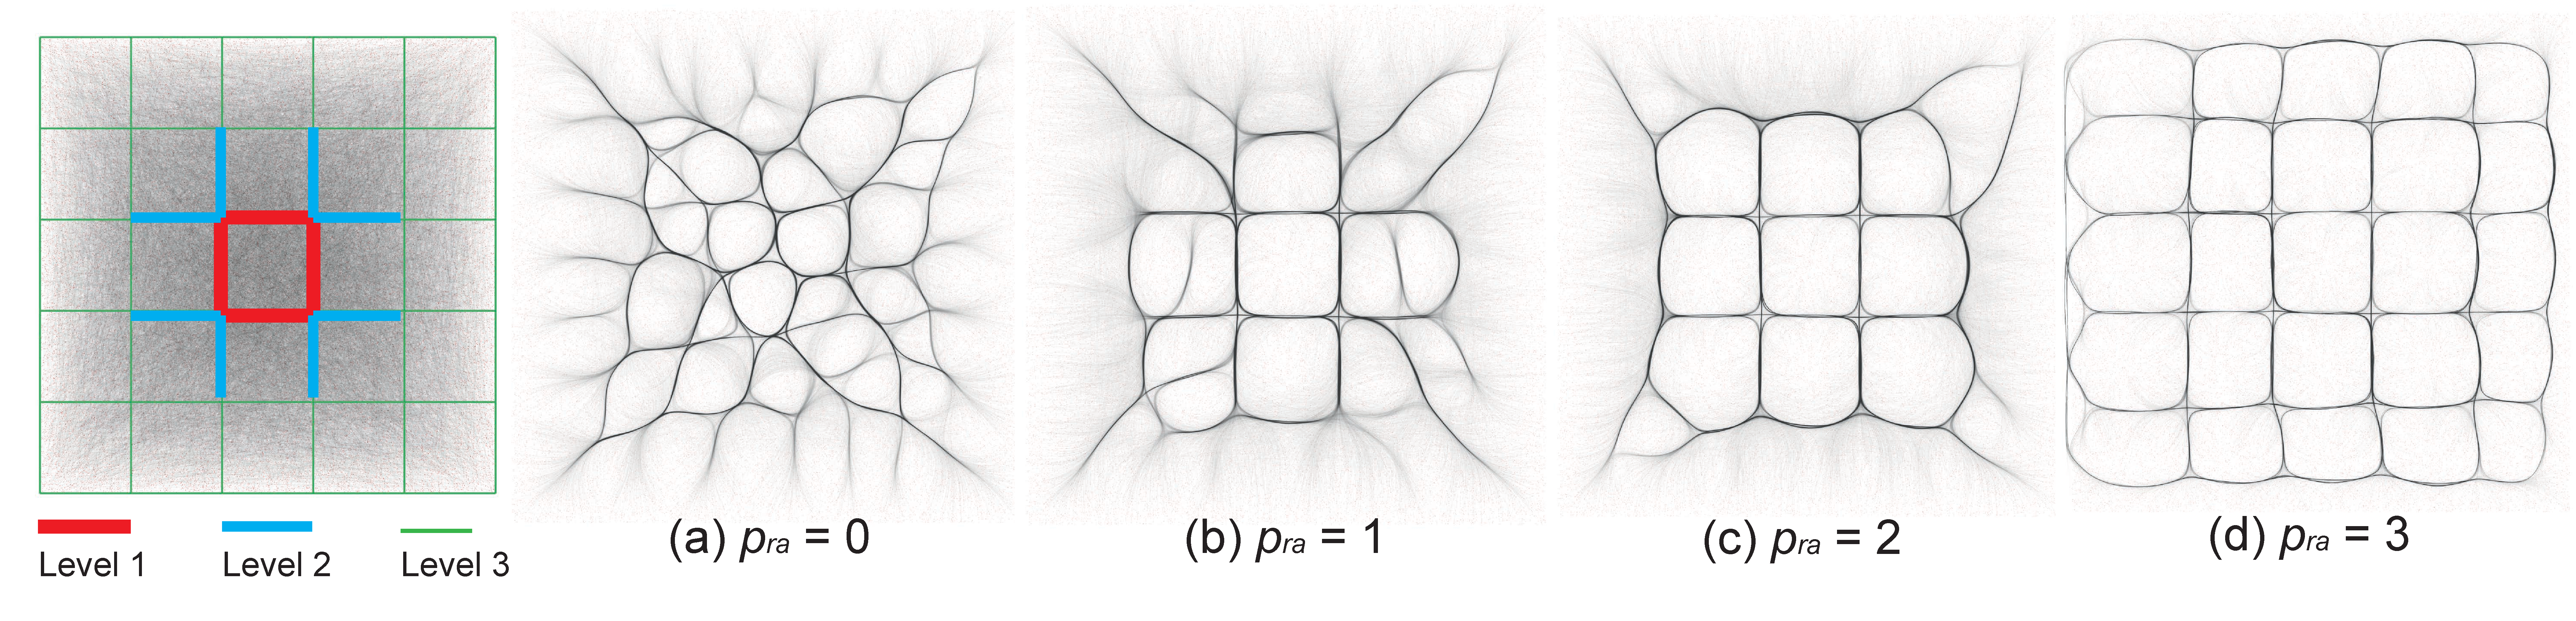
\includegraphics[width=0.995\textwidth]{figure/edgebundling/fig6_grid/route}
	\vspace{-4mm}
	\caption{
		Leftmost: raw 100K artificial OD trails on a grid road network in there hierarchies. 
		(a) - (d): RAEB bundling results with route awareness parameter $p_{ra}$ set to 0 - 3, respectively.
		}
	\label{fig:grid}
	\vspace{-4mm}
\end{figure*}
%%%%%%%%%%%%%%%%%%%%%%%%%%%%%%%%%%%%%%%%%%%%%%%%%%%%%%%%%%%%%%%%%%%%%%%%%%%%%%%%%%%%%%%%%%%%%%%%%%
%%%%%%%%%%%%%%%%%%%%%%%%%%%%%%%%%%%%%%%%%%%%%%%%%%%%%%%%%%%%%%%%%%%%%%%%%%%%%%%%%%%%%%%%%%%%%%%%%%

We employ mutual information (MI) - a basic concept from information theory, as a quantitative indicator for measuring bundling stability.
Maes et al.~\cite{maes1997multimodality} introduced MI to measure statistic dependence between intensities of corresponding voxels in two medical images.
This work measures MI between images generated in consecutive bundling iterations, which are geometrically aligned.
Hence, the measurement is simplified without geometry matching. 
Let denote two input images $X$ and $Y$.
MI is computed as:

\vspace{-2mm} 
\begin{equation} \label{eq:mi}
I(X, Y) = \sum_{x}\sum_{y}p(x,y)log(\frac{p(x,y)}{p(x)p(y)}))
\end{equation}

\noindent
where $p(x)$ and $p(y)$ indicate the intensity at $x \in X$ and $y \in Y$, and $p(x, y)$ measures the joint value between $p(x)$ and $p(y)$.
MI is affected by image size, while we prefer a constant measurement for different graph drawings.
Hence, we adopt normalized MI (NMI):

\vspace{-2mm} 
\begin{equation}\label{eq:nmi}
NMI(X, Y) = \frac{2I(X,Y)}{H(X) + H(Y)} 
\end{equation}

\noindent
where $H(X) = -\sum p(x)log(p(x)))$ that measures entropy for $X$.

We introduce a new parameter of bundling stability $p_{bs}$.
$p_{bs}$ is computed in every iteration as NMI($I_n$, $I_{n-1}$), where $I_n$ and $I_{n-1}$ denote images generated at iteration $n$ and $n-1$, respectively.
Figure~\ref{fig:nmi}(left) presents NMIs at each bundling iteration for three different kernel size decay ratios $\lambda$.
It is observed that NMI increases when bundling iteration increases, and smaller $\lambda$ leads to faster NMI increment.
All NMIs pass over 0.75 around iteration 10, and reach close to 0.8 at iteration 15.
Figure~\ref{fig:nmi}(right) shows two images at iteration 10 and 11 for $\lambda$ = 0.9.
The images are hardly distinguishable from each other.
Thus, we can claim the bundling produces stable results, and the process can terminate.
In this way, we determine a threshold for $p_{bs}$ to control bundle termination.
If a bigger threshold is chosen, more stable results will be generated.

%%%%%%%%%%%%%%%%%%%%%%%%%%%%%%%%%%%%%%%%%%%%%%%%%%%%%%%%%%%%%%%%%%%%%%%%%%%%%%%%%%%%%%%%%%%%%%%%%%
\subsection{Bundle Deviation}
$p_{bs}$ is introduced for measuring visual stability of bundle layouts generated by one bundling method.
However, $p_{bs}$ is not suitable for comparing bundling quality of multiple bundling methods.
Many evaluation metrics can be used for comparing graph layouts, such as edge crossing, ambiguity, and edge direction.
These metrics are suitable for general graphs without a ground truth.
However, OD trails studied in this work are constrained in roads in a city.
We would like to keep the generated bundles close to their OD trails on the road network.
Though map matching algorithm can intrdouces errors, this work treats mapped OD trails as ground truth, instead of raw OD trails.
This is because of: for \textit{UT-1} urban traffic, only origin and destination information are recorded; for \textit{UT-2} urban traffic, accuracy of GPS positions are not perfect.

We introduce a new parameter of bundle deviation, denoted as $p_{d}$, to measure distance between final bundles and OD trails mapped on the road network.
Both bundles and OD trails can be modeled as polylines made up of sequential positions in geographical space.
Thus, the distance between them can be measured using discrete Frechet Distance.
We calculate mean distances for all bundles, and map the mean in graph drawing space.